% Algorithms ~ A. Labouseur, Assignment 3 - Connor Fleischman

\documentclass[12pt, letterpaper]{article}
\usepackage{graphicx} % Required for inserting images
\usepackage{listings} % Required for inserting code
\usepackage{xcolor} % Required for formatting code
\usepackage{fancyhdr} % For custom headers and footers
\usepackage{titlesec} % For enhanced section titles
\usepackage{mathpazo} % For elegant fonts
\usepackage{tocloft} % For custom table of contents
\usepackage{appendix} % For appendices
\usepackage{hyperref} % For clickable links in TOC
\usepackage{amsmath, amssymb}
\usepackage{geometry}
\usepackage{bookmark}

\graphicspath{{./report/figures/}}
\lstset{language=C++, inputpath=./src/}
\geometry{a4paper, margin=1in}

% Custom Colors
\definecolor{background}{rgb}{0.84,0.84,0.84}
\definecolor{codegreen}{rgb}{0.2,0.7,0.2}
\definecolor{codeblue}{rgb}{0,0,0.7}
\definecolor{codegray}{rgb}{0.5,0.5,0.5}
\definecolor{codepurple}{rgb}{0.58,0,0.82}
\definecolor{codered}{rgb}{0.6,0,0}
\definecolor{keywordcolor}{rgb}{0.6,0,0.6}

% Custom Header and Footer
\pagestyle{fancy}
\fancyhf{}
\fancyhead[L]{\textit{Connor Fleischman - Assignment 3}}
\fancyhead[R]{\textit{Algorithms | Dr. Labouseur}}
\fancyfoot[C]{\thepage}
\setlength{\headheight}{14.5pt}


% Section Title Customization
\titleformat{\section}[block]{\Large\bfseries\color{black}}{\thesection}{1em}{}

% TOC (Link) Customization
\renewcommand{\cftsecfont}{\bfseries}
\renewcommand{\cftsecpagefont}{\bfseries}

% Define and set my code style
\lstdefinestyle{mystyle}{
   backgroundcolor=\color{white},   
   commentstyle=\color{blue},
   keywordstyle=\color{purple}\bfseries,
   numberstyle=\tiny\color{black},
   stringstyle=\color{gray},
   basicstyle=\ttfamily\tiny,
   frame=single, 
   rulecolor=\color{black},
   breakatwhitespace=false,         
   breaklines=true,                 
   captionpos=b,                    
   keepspaces=true,                 
   numbers=left,                    
   numbersep=10pt, 
   showspaces=false,                
   showstringspaces=false,
   showtabs=false,                  
   tabsize=4,
   emph={int,char,double,float,unsigned}, 
   emphstyle={\color{blue}},
}

\lstset{style=mystyle}

% Document Title and Metadata
\title{Assignment 3 - LaTeX Write-Up}
\author{Connor Fleischman}
\date{November 15, 2024}

% \begin{document}
\begin{document}

% Title Page
\pagenumbering{roman} % Start page numbering in i, ii..
\maketitle
\begin{center}
   
\includegraphics[width=120mm,scale=0.5]{MaristSeal.png}
\end{center}
\newpage

% Table of Contents
\tableofcontents
\newpage
\setcounter{page}{1} % Start page numbering at 1
\pagenumbering{arabic} % Start page numbering in 1, 2..

\section{Introduction}
\textbf{Assignment 3} focuses on the design and implementation of multiple Undirected Graphs (\ref{Graph}), a Binary Tree (\ref{BST}), and computing their performances in the context of the assignment.
Specifically, to create a program which can \textit{dynamically read and interpret} a blueprint of multiple graphs.
Create these graphs, returning their matrix, adjacency list, and performing a depth-first and breadth-first traversal of the graph.
\vspace*{5px}
\newline
\textit{Dynamic reading \& interpretation}: A way of building your code by avoiding hard-coding, to allow any form of input, following some syntactical rules, to be read and interpreted. 

\section{Undirected Graphing} \label{Graph}
The first of \textbf{Assignment 3}'s goals was to develop several implementations of Undirected Graphs from the data in \texttt{graphs1.txt}
\vspace*{5pt}
\newline
This will include:
\begin{itemize}
   \item Parsing \texttt{graph1.txt} into individual graphs
   \item Building the graph of linked objects
   \item Perform operations on the graph
   \item Graph deletion
   \item Building the next graph
   \item Go back to step 2 if not finished $\langle \langle Recurse! \rangle \rangle$
\end{itemize}
For each graph representation, we will perform operations such as printing the matrix (\ref{Matrix}) and adjacency lists (\ref{AdjList}), a depth-first and breadth-first traversal (\ref{Traversals}), and a deletion of the graph, its vertices and edges.

\subsection{Matrix} \label{Matrix}
A matrix is a 2D array where rows and columns represent vertices.
Each cell indicates the presence of an edge between two vertices.
A matrix is properly implemented if it has mirror symmetry along its diagonal.
In \textbf{Assignment 3} we were to create and display a matrix for every graph provided in \texttt{graph1.txt}
\subsubsection{Implementation}
\begin{center}
   \lstinputlisting[language=C++, caption=Matrix Implementation, firstline=205, lastline=253]{graph/UndirectedGraph.h}
\end{center}
As we see above, a flag is used to record if the nested for i, j loop crosses two vertices whom are neighbors.
If they are neighbors an 'X' is recorded at that position in the grid, if no neighbor is present a '-' is noted.
Most of the complexity in this section results from the formatting of the matrix in a legible and clean way.
\subsubsection{Results}
\begin{center}
   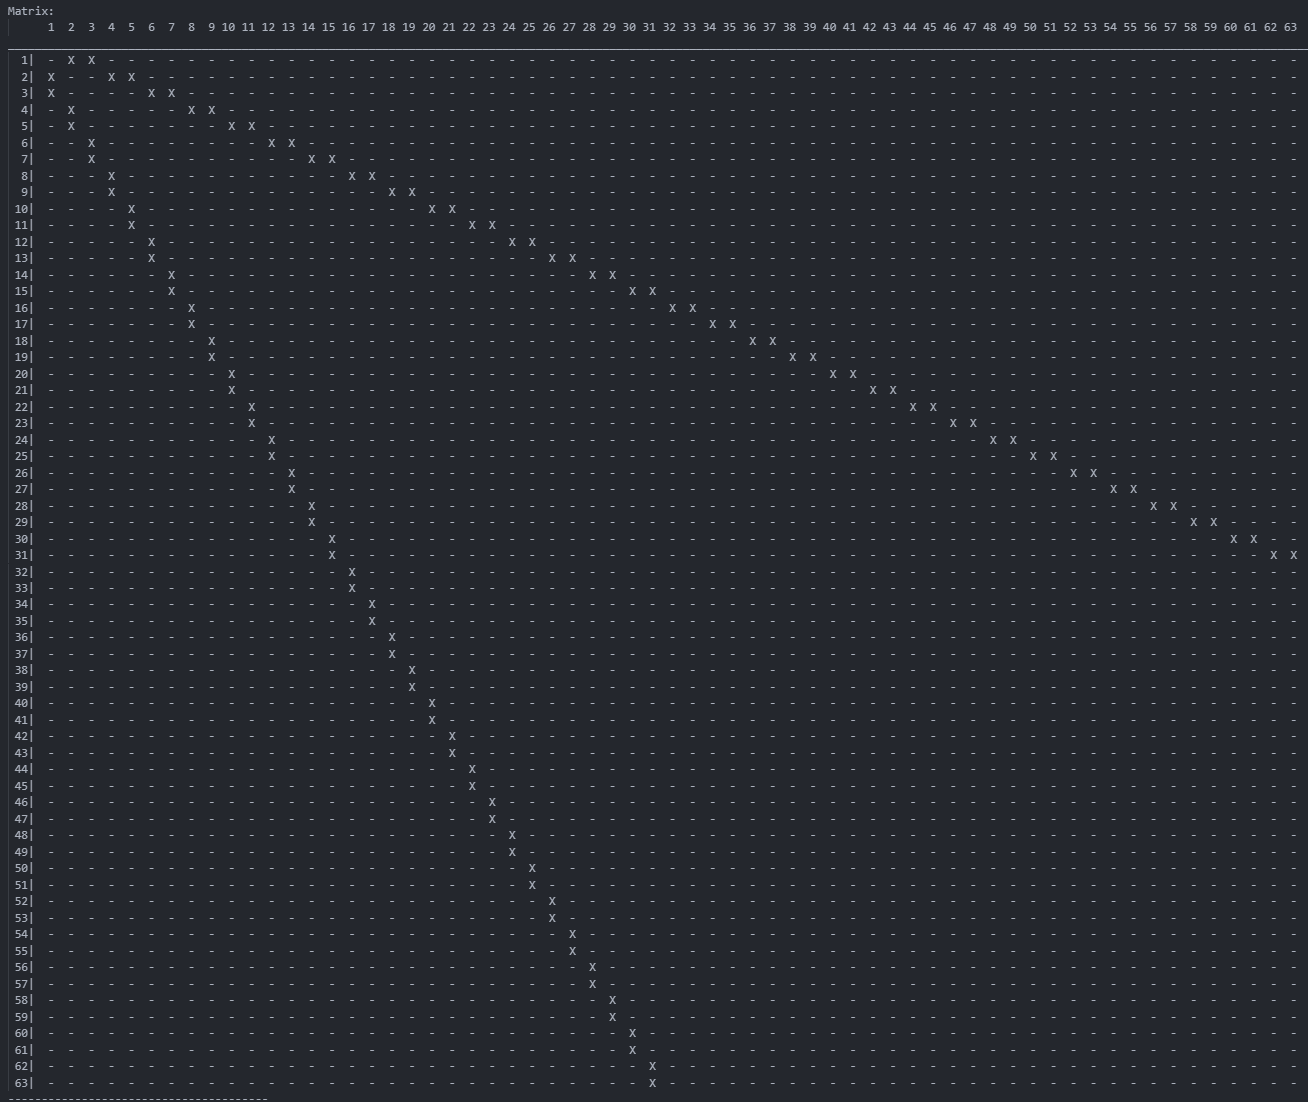
\includegraphics[width=120mm,scale=0.5]{Images/Graph3_Matrix.png}
\end{center}
As a stylistic and space-efficient choice I will not include every output of every graph in \texttt{graph1.hs}
However, I'd be remiss if I could not brag about my output.
As we can see above, mirror symmetry along the diagonal depicts this graph, Graph \#5 in the file, with 63 vertices.
With a matrix it is very easy to notice patterns in the connections of a graph's edges.

\subsection{Adjacency List} \label{AdjList}
An adjacency list stores lists of neighboring vertices for each vertex.
These are useful in quickly identifying disconnected vertices and which have the most neighboring vertices.
In \textbf{A3}, similarly to the matrix, for every graph we display it as an adjacency list.
\subsubsection{Implementation}
\begin{center}
   \lstinputlisting[language=C++, caption=Adjacency List Implementation, firstline=182, lastline=203]{graph/UndirectedGraph.h}
\end{center}
The code above is fairly straightforwards. It simply returns every vertex in the graph and its neighbors.
An adjacency list is useful in many cases, for example:
\begin{itemize}
   \item Shortest Path Algorithms
   \subitem Allows for full exploration of each vertex's edges
   \item Social Network Analysis
   \subitem Where users represent vertices and each friendship is an edge
\end{itemize}
\subsubsection{Results}
\begin{center}
   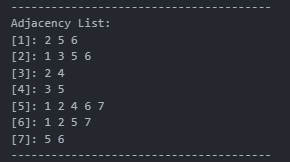
\includegraphics[width=120mm, scale=0.5]{Images/Graph1_AdjList.png}
\end{center}
This is the Adjacency List created for graph \#1.
It is a very boring list but some information can be gathered.
First, we can note the \textit{independent sets} within the graph and \textit{maximum independent set}.
And because you can find the \textit{independent sets}, means you can find the \textit{vertex cover} (and \textit{optimal vertex cover}).
\vspace*{5px}
\newline
\textit{Independent Set}: A subset of all vertices such that for every vertex in the graph, it has no neighbors whom are neighbors of any other vertex in the graph
\vspace*{5px}
\newline
\textit{Maximum Independent Set}: An independent set of the largest possible cardinality
\vspace*{5px}
\newline
\textit{Vertex Cover}: A subset of all vertices such that the sum of all vertices's neighbors must total all vertices.
I.e., the graph above has a vertex cover of [2,4,5,6] 
\vspace*{5px}
\newline
\textit{Optimal Vertex Cover}: A vertex cover of maximum size for the given graph

\subsection{Traversal Analysis} \label{Traversals}
\textbf{Depth-First Search (DFS)}:
\newline
A depth-first traversal performed on an undirected graph has a time complexity of $O(V + E)$.
The recursion stack for DFS may be up to $O(V^2)$ in the worst case.
This is because if every vertex has an edge to every vertex then it would be $O(V + V) = (V^2)$.
\subsubsection{DFS Implementation}
\begin{center}
   \lstinputlisting[language=C++, caption=DFS Traversal Implementation, firstline=34, lastline=48]{graph/UndirectedGraph.h}
\end{center}
When performing a depth-first traversal, intuitively, you have to go as deep as possible first.
We do this through recursion, by recursively calling our traversal function on itself until reaching all vertices, we effectively travel to all neighbors from the deepest first.
\vspace*{5px}
\newline
\textbf{Breadth-First Search (BFS)}:
\newline
Breadth-first traversal also runs in $O(V + E)$.
It uses a queue data structure to keep track of the nodes to visit.
This can result in the same $O(V^2)$ performances. 
However a queue to not suffer from recursive loops causing stack overflow errors used rather than the stack.
\subsubsection{BFS Implementation}
\begin{center}
   \lstinputlisting[language=C++, caption=BFS Traversal Implementation, firstline=50, lastline=70]{graph/UndirectedGraph.h}
\end{center}
When performing a breadth-first search our goal is to go wide before deep.
So in order to achieve this on a graph without a hierarchy, since it is more simple on trees, we use a queue to maintain the sequence of traversal.
Through this, we can search all the neighbors of a vertex before traversing to all the neighbors of the first neighbor of the first vertex.
\subsubsection{Results}
\begin{center}
   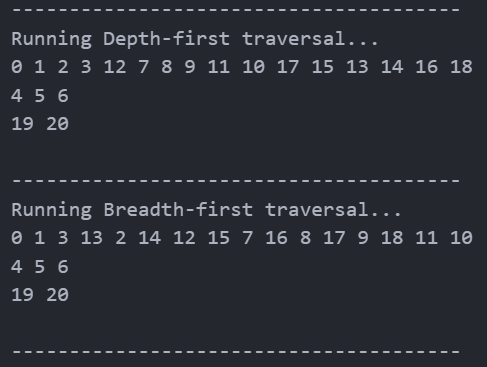
\includegraphics[width=100mm, scale=0.5]{Images/Graph5_Traversals.png}
\end{center}
In the above image we see the Depth-first and Breadth-first traversals on Graph \#5.
I chose to include this graph specifically because of its disconnected vertices.
It is important to remember to search all vertices, not just neighboring ones while traversing.

\section{Binary Search Tree (BST)} \label{BST}
The second goal in \textbf{Assignment 3} was to construct a Binary Tree, where each node has either 0, 1, or 2 children, no more, parsing the data from \texttt{magicItems.txt}
\vspace*{5pt}
\newline
This will include:
\begin{itemize}
   \item Parsing \texttt{magicItems.txt}
   \item Inserting each item into the tree, recording its path from root to its place
   \item Parsing recording each key in \texttt{magicitems-find-in-bst.txt}
   \item Perform operations on the tree
   \item Record data on these operations
   \item Tree deletion
\end{itemize}
We perform an in-order depth-first traversal on the tree (\ref{Trav}), once all 666 items are inserted (\ref{Insert}).
Since we insert items with the least on the left and most on the right, this results in an output of the items in alphabetical order.
We also perform searches for 42 keys provided (\ref{Search}), for each search we compute the number of comparisons made when traversing the tree to find the node (from the root down).
Then, after all 42 keys have been searched, regardless of if the item was found, we compute the total average number of comparisons required for a key in the tree.

\subsection{Item Insertion} \label{Insert}
Once the \texttt{magicItems.txt} file is parsed it is then inserted line by line into the Binary Search Tree.
I don't think anyone wants to see 666 items going into the tree so heres only the first few.
\subsubsection{Results}
\begin{center}
   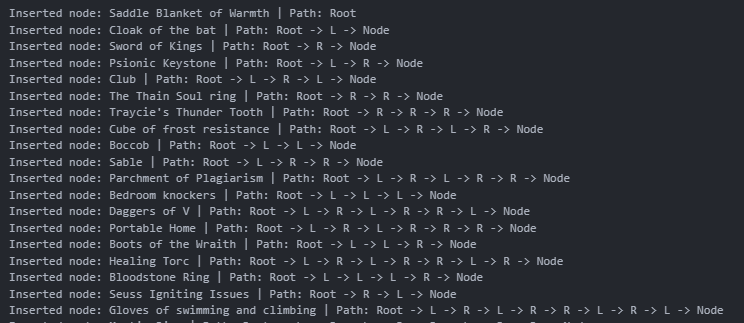
\includegraphics[width=120mm, scale=0.5]{Images/BinTree_InsertStart.png}
\end{center}
And the last few.
\begin{center}
   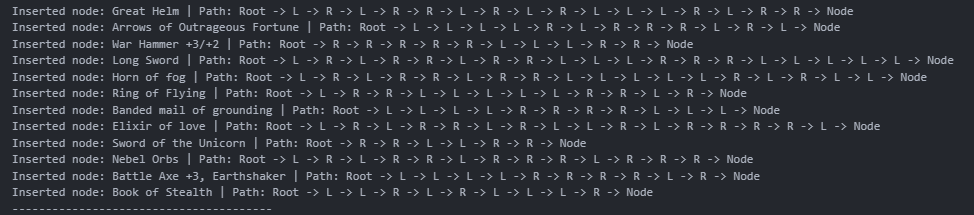
\includegraphics[width=120mm, scale=0.5]{Images/BinTree_InsertEnd.png}
\end{center}
We can see that the code inserts all 666 items to its proper position, while recording its path from root to its position.
\subsubsection{Insertion Implementation}
\begin{center}
   \lstinputlisting[language=C++, caption=Item Insertion Implementation, firstline=42, lastline=91]{tree/BinaryTree.h}
\end{center}
This code handles the insertion of nodes into the tree.
After handling weather or not the graph is empty and if there needs to be a root added, a while loop is created which traverses the tree until finding the deepest position.
As the loop traverses, the path of the node to be inserted is updated if we traverse a left-child or right-child.
Finally it records the node insertion and its path if it was successfully inserted.

\subsection{In-Order Traversal} \label{Trav}
An in-order traversal of a BST gives the elements in sorted order.
This is an extremely useful traversal since an in-order traversal of a Binary Tree outputs the items in a sorted order of least to greatest.
\subsubsection{Traversal Implementation}
\begin{center}
   \lstinputlisting[language=C++, caption=In-order Traversal Implementation, firstline=146, lastline=161]{tree/BinaryTree.h}
\end{center}
Here we perform an in-order depth-first traversal of the Binary Tree.
As explained earlier in the Binary Search Tree section (\ref{BST}), when we run this, we should get back a sorted traversal of the items in alphabetical order.
\subsubsection{Results}
Below is the traversal output:
\begin{center}
   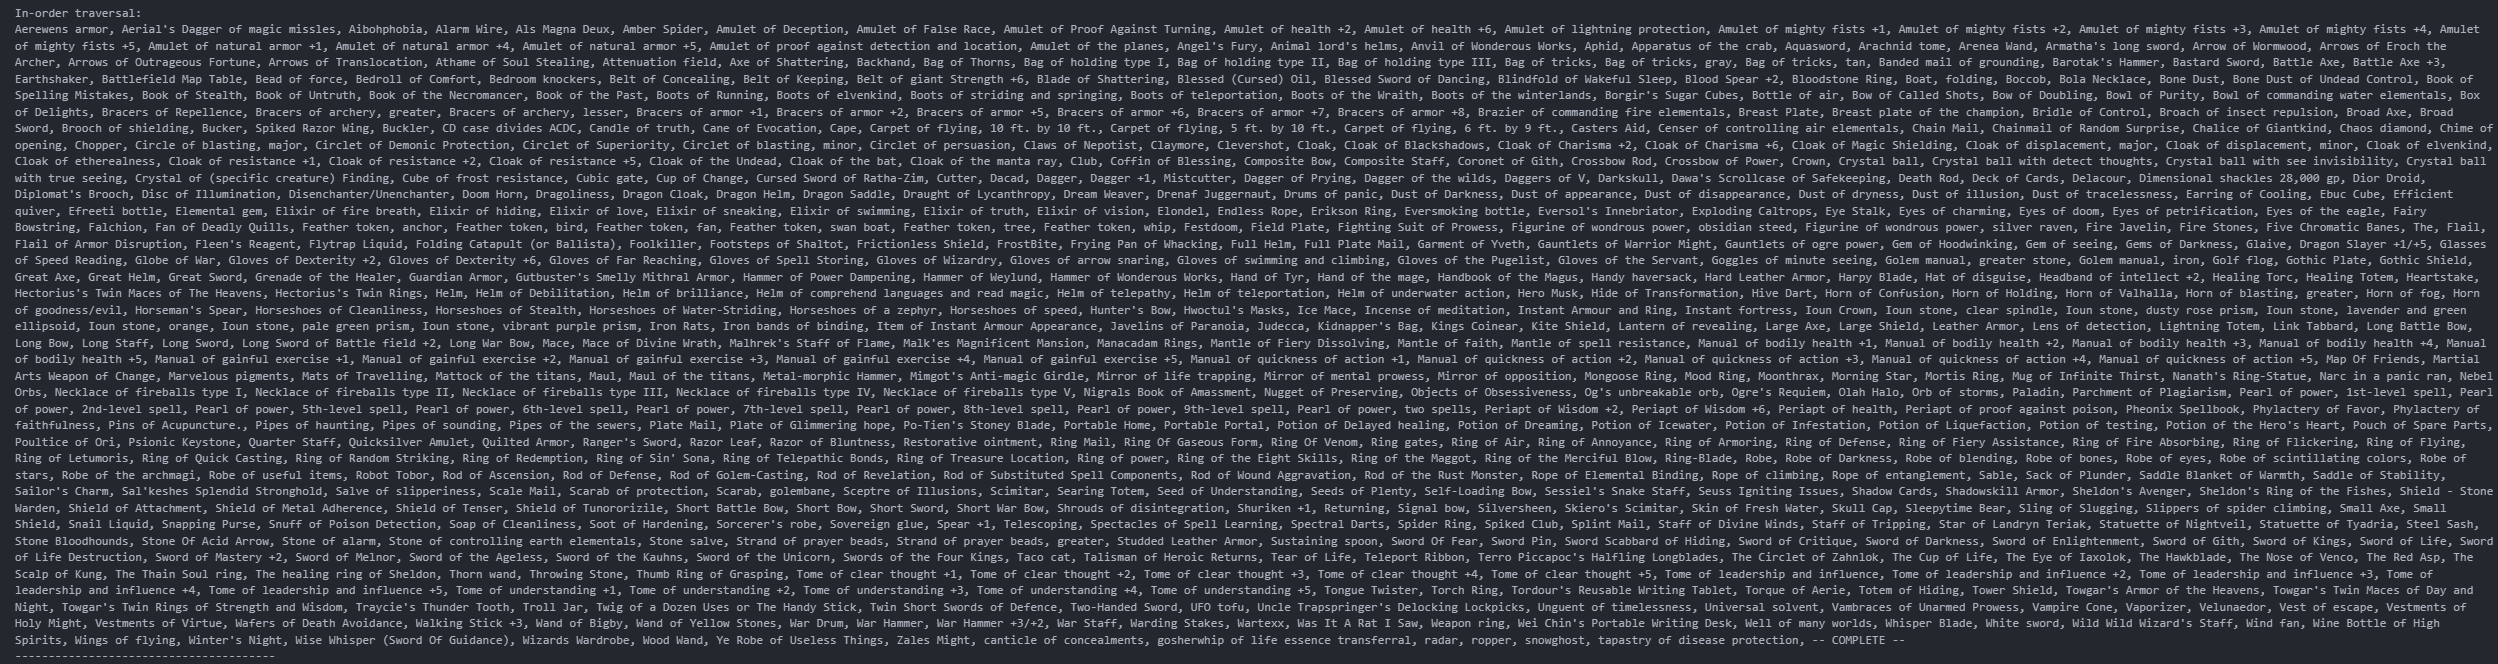
\includegraphics[width=120mm, scale=0.5]{Images/BinTree_Traversal.png}
\end{center}

\subsection{Look-up Analysis} \label{Search}
When looking up items from \texttt{magicitems-find-in-bst.txt}, we recorded the path and the number of comparisons.
The average time complexity of searching in a BST is $O(\log n)$, assuming the tree is balanced.
However, in the worst case (e.g., if the tree becomes a linked list), the complexity degrades to $O(n)$.
This can happen if the tree is sorted before being inserted.
\subsubsection{Results}
\begin{center}
   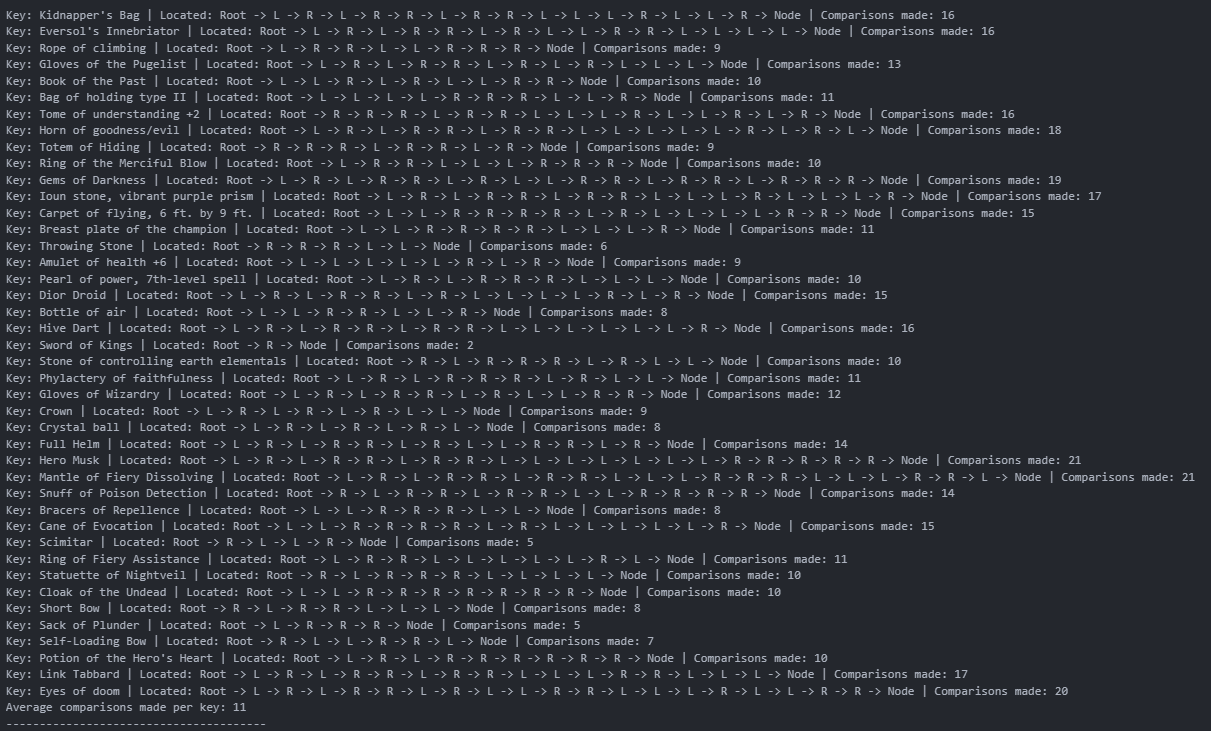
\includegraphics[width=120mm, scale=0.5]{Images/BinTree_Searches.png}
\end{center}
As we can see in the picture, the average look-ups required per search was 11.
This is within the range of expected number of comparisons.
\subsubsection{Look-up Implementation}
\begin{center}
   \lstinputlisting[language=C++, caption=Search Implementation, firstline=163, lastline=187]{tree/BinaryTree.h}
\end{center}
The above code performs a search.
Given some nodes ID (as a string), and searches for the first node with the same in the vertices.
Then returns its path along with the number of comparisons needed to find it.

\appendix
\section{Conclusion}
In this assignment, we explored different ways to represent and manipulate graph data structures and implemented a binary search tree.
Each representation has its pros and cons, depending on the density of the graph and the types of operations performed.

\end{document}
